
\subsection{Maximum {\em A Posteriori} Adaptation}
\label{sec:adaptation}

Our ASR framework is based on weighted finite-state transducers (WFSTs) as outlined in~\cite{mohri2008speech}. 
In this framework, the acoustic model is specified by a probabilistic mapping from acoustic signals to a sequence of discrete symbols, and a WFST $H$ mapping these symbol sequences to triphone sequences. The other WFSTs in the framework are $C$ which maps down triphone sequences to monophone sequences, a pronunciation model $L$ and a language model $G$. Since our tasks involve phone recognition, $L$ is essentially an identity mapping and $G$ is a phone N-gram model. 

To describe the adaptation process, it will be helpful to compare the following two cases.
\begin{itemize}
\item In training the parameters of the baseline acoustic model, for each training utterance, we work with the cascade $H \circ C \circ L \circ T$, where $T$ is a linear chain FST representing the training transcript. The multilingual baselines described in Section~\ref{sec:mlbaseline} are trained in this manner using training data from languages other than the target language.

  Here, the parameters are updated using Viterbi training which computes maximum likelihood estimates based on the best path through the cascade.

\item During adaptation, for each training utterance (in the target language), we work with the cascade $H \circ C \circ L \circ PT$, where $PT$ is a WFST representing the probabilistic transcript, obtained as in Section~\ref{sec:MC}.

Here, we use maximum a posteriori (MAP) estimation to update the parameters. Further, as explained below, a lattice derived from the cascade is used instead of a single path.
\end{itemize}

%% wrong figure reference?  Shouldn't this be fig:pt ?
As noted in Figure~\ref{fig:listPER}, a PT contains significant amount of information beyond any single transcript extracted from the PT. Motivated by this, the statistics for the MAP estimation are accumulated from a lattice derived from the cascade $H \circ C \circ L \circ PT$, rather than reducing the PT to its single best path.

Though it is disadvantageous to reduce a PT to its best path, it is
nevertheless advantageous to incorporate as much information as
possible from the language model during adaptation.  Composing $L\circ
PT$ is complicated, however, by the presence of null transitions in
the PT.  A null transition in the PT matches a non-event in the
language model, for which normal FST notation has no representation.
In order to compose the PT with the language model, therefore, it is
necessary to introduce a special type of ``non-event'' symbol, here
denoted ``\#2'', into the language model (Fig.~\ref{fig:liu1}).  As
shown in Fig.~\ref{fig:liu1}, a language model ``non-event'' is a
transition that leaves any state, and returns to the same state (a
self-loop).  Such self-loops, labeled with the special symbol ``\#2''
on both input and output language, are added to every state in the
phonotactic language model (left-hand side of Fig.~\ref{fig:liu1}).
The probabilistic transcript, then, is augmented with the special
symbol ``\#2'' as the input-language symbol for every null-output edge
(output symbol is $\phi_m^\ell =\epsilon$).

\begin{figure}
  \centerline{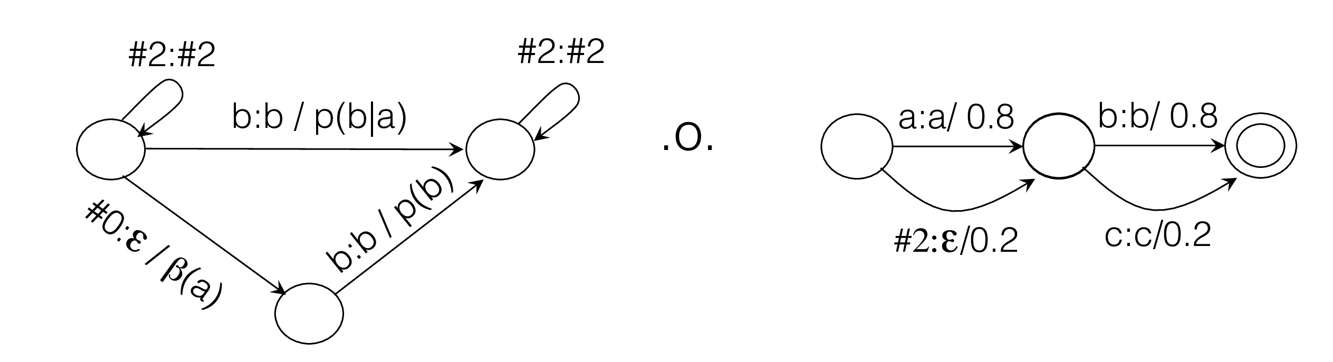
\includegraphics[width=5in]{../figs/liu1.png}}
  \caption{Deletion edges in the probabilistic transcript (edges with
    the special null output symbol, $\epsilon$), required special
    handling in order to use information from a phonotactic language
    model.  As shown, a new type of null symbol, ``\#2'', was invented
    to represent the input for every PT edge with an $\epsilon$ output
    (right).  Such edges were only allowed to match with state
    self-loops, newly added to the language model (left) in order to
    consume such non-events in the transcript.}
  \label{fig:liu1}
\end{figure}

The Bayesian framework for maximum {\em a posteriori} (MAP) estimation has
been widely applied to GMM and HMM parameter estimation problems such
as parameter smoothing and speaker
adaptation~\cite{gauvain1994maximum}.
%% single-sentence paragraph. consider merging with following paragraph.

Formally, for an unseen target language, we denote its acoustic observations $\mathbf{x}= ( x_1, \ldots, x_{T} )$, and its acoustic model parameter set as $\lambda$, then the MAP parameters are defined as:
%
\begin{equation}
  %\begin{split}
    \lambda_{\mathrm{MAP}}  = \argmax_{\lambda} \Pr(\lambda | \mathbf{x}) 
= \argmax_{\lambda} \Pr( \mathbf{x} | \lambda ) \Pr(\lambda)
%\end{split}
\label{eq:map}
\end{equation}
%
\noindent where we use multilingual baseline GMM-HMM parameters to assign the conjugate prior hyperparameters in $\rho(\lambda)$, and take the modes of the prior distributions as the initial model parameter estimates. Using suitable models for these distributions,  \cite{gauvain1994maximum} derive update rules in an EM algorithm for computing $\lambda_{\mathrm{MAP}}$. For example, the mean $\mu_{ik}$ of the GMM mixture component $k$ associated with HMM state $i$ is updated as:
\begin{align}
\tilde{\mu}_{ik} &= \frac{\tau_{ik} \mu_{ik} + \alpha_{ik} \hat{\mu}_{ik} }{\tau_{ik}  + \alpha_{ik}  } \\
\alpha_{ik}= \sum_{t=1}^{T} c_{ikt}  &\qquad\qquad\qquad
\hat{\mu}_{ik} = \frac{ \sum_{t=1}^{T} c_{ikt} x_t }{ \sum_{t=1}^{T} c_{ikt}  } \notag
\end{align}
where $\tau_{ik}$ is a hyperparameter in the prior density for the mixture component $k$ of state $i$  and $c_{ikt}$ denotes the probability of the HMM being in state $i$ with mixture component $k$ given observation $x_t$ (estimated using statistics accumulated from the cascade $H \circ C \circ L \circ PT$).  Here, $\hat{\mu}_{ik}$ is the maximum likelihood estimate of $\mu_{ik}$ given the target language data $\mathbf{x}$ and the model parameters $c_{ikt}$. Note that at each step of the iteration, $\tilde{\mu}_{ik}$ linearly interpolates between $\mu_{ik}$ and $\hat\mu_{ik}$.
In our setting,  the initial value of $\mu_{ik}$ is obtained from the multilingual baseline model, and $\tilde{\mu}_{ik}$ eventually converges to a model for the target language data.

The baseline and the adapted models were implemented using Kaldi~\cite{Kaldi2011}. In order to efficiently carry out the required operations on the cascade $H \circ C \circ L \circ PT$, we carefully designed $PT$ as an acceptor defined as $\mathrm{proj}_{\mathrm{input}} (\widehat{PT})$, where $\widehat{PT}$ is a WFST mapping phone sequences to English letter sequences obtained as a cascade of WFSTs modeling the distributions shown in Equation~\ref{eq:PT}, and $\mathrm{proj}_{\mathrm{input}}$ refers to projecting onto the input labels. For the purposes of computational efficiency, the cascade for $\widehat{PT}$ includes an additional WFST restricting the number of consecutive deletions of phones and insertions of letters (to a maximum of 3 in our experiments). We use two additional disambiguation symbols~\cite{mohri2008speech}, apart from the ones used in typical Kaldi recipes, to determinize these insertions and deletions in $\widehat{PT}$. MAP adaptation for the acoustic model was carried out for a number of iterations (12 for yue \& cmn, 14 for hun \& swh, with a re-alignment stage in iteration 10).
%% I think there is need for a short section that
%% comes between sections 2 and 3 that explains the big picture of what
%% was done, in broad strokes, before getting into the mathematical
%% details of how the system was designed. Perhaps under the heading of
%% "Overview of experimental procedures" or similar.
%% 
%% Second comment: This is the first mention of the particular training 
%% languages used in these experiments. The abbreviations have not been
%% introduced yet.
%% That said, I'm not sure that this point in the manuscript is the right
%% place for this particular detail of the implementation (how many
%% iterations were done for each training language). So far the rest of
%% section 3 has been about fundamental system design details that are
%% unrelated to the particular choice of training languages. I suggest
%% moving this detail to the "Experimental Methods" section. If it's
%% really necessary to mention it here, perhaps it could just say:
%% "A variable number of iterations of the MAP adaptation were carried
%% out for the different training languages (see Section XXX for details)."
